\chapter{Introduction}

%\chapter*{Introduction}
\label{intro}

% \par Introducere: obiectivele lucrarii si descrierea succinta a capitolelor, prezentarea temei, prezentarea contributiei proprii, respectiv a rezultatelor originale si mentionarea (daca este cazul) a sesiunii de comunicari unde a fost prezentata sau a revistei unde a fost publicata.
%THEME PRESENTATION
\section{Understanding Depression: Statistics and Insights}
\label{sec:ch1sec1}

\par \quad Depression stands as a prevalent mental health affliction with profound impacts on both psychological and physical well-being. Characterized by a disinterest in routine activities, sleep disturbances, anhedonia, and in severe cases, suicidal ideation \cite{cui2015systematic}, it has become a pervasive chronic ailment across global societies, disrupting functionality, engendering despondency, and diminishing life quality. Furthermore, individuals grappling with major depressive disorder face heightened susceptibility to cardiovascular ailments, suboptimal treatment outcomes, and elevated rates of morbidity and mortality \cite{seligman2015interface,luo2018effects}.

The World Health Organization (WHO) identifies depression as the primary contributor to global disability, affecting over 300 million individuals worldwide \cite{smith2014world}. Particularly alarming is the revelation that adolescents with severe depression are 30 times more prone to suicide \cite{stringaris2017depression}. Despite its recognized significance as a global health challenge, the intricate mechanisms underlying depression's etiology remain inadequately elucidated, albeit cultural, psychological, and biological factors are acknowledged as contributors \cite{gross2014silver,menard2016pathogenesis}.

The Global Burden of Disease (GBD) study \cite{liu2020changes} offers comprehensive insights into various ailments across 195 countries, including depression. Divided into dysthymia and major depressive disorder categories, the GBD database from 1990 to 2017 furnishes valuable data for understanding depression's prevalence trends globally. Major depressive disorder emerges as a predominant form of depression, posing a significant burden on global health, with projections indicating it may become the leading cause of disability by 2030. Moreover, while dysthymia rates decreased in some regions, it remains a concern, particularly in the United States.

Identifying underlying causes and risk factors for depression, including genetic predisposition, demographic factors, unhealthy lifestyles, and comorbidities such as stroke, cancer, and AIDS, underscores the need for multifaceted interventions and targeted policies. Governments in countries with high depression rates are urged to prioritize research, promote healthy lifestyles, and ensure comprehensive care for individuals with predisposing conditions. However, the study acknowledges limitations in data analysis, advocating for future research to delve deeper into regional risk factors and guide tailored policy interventions for effective depression control globally, As seen in Figure \ref{FigGloablDepression} \cite{liu2020changes}, which evaluated the worldwide burden of depression using the estimated annual percentage change (EAPC) and age-standardized incidence rate (ASR).

\begin{figure}[htbp]
	\centering
		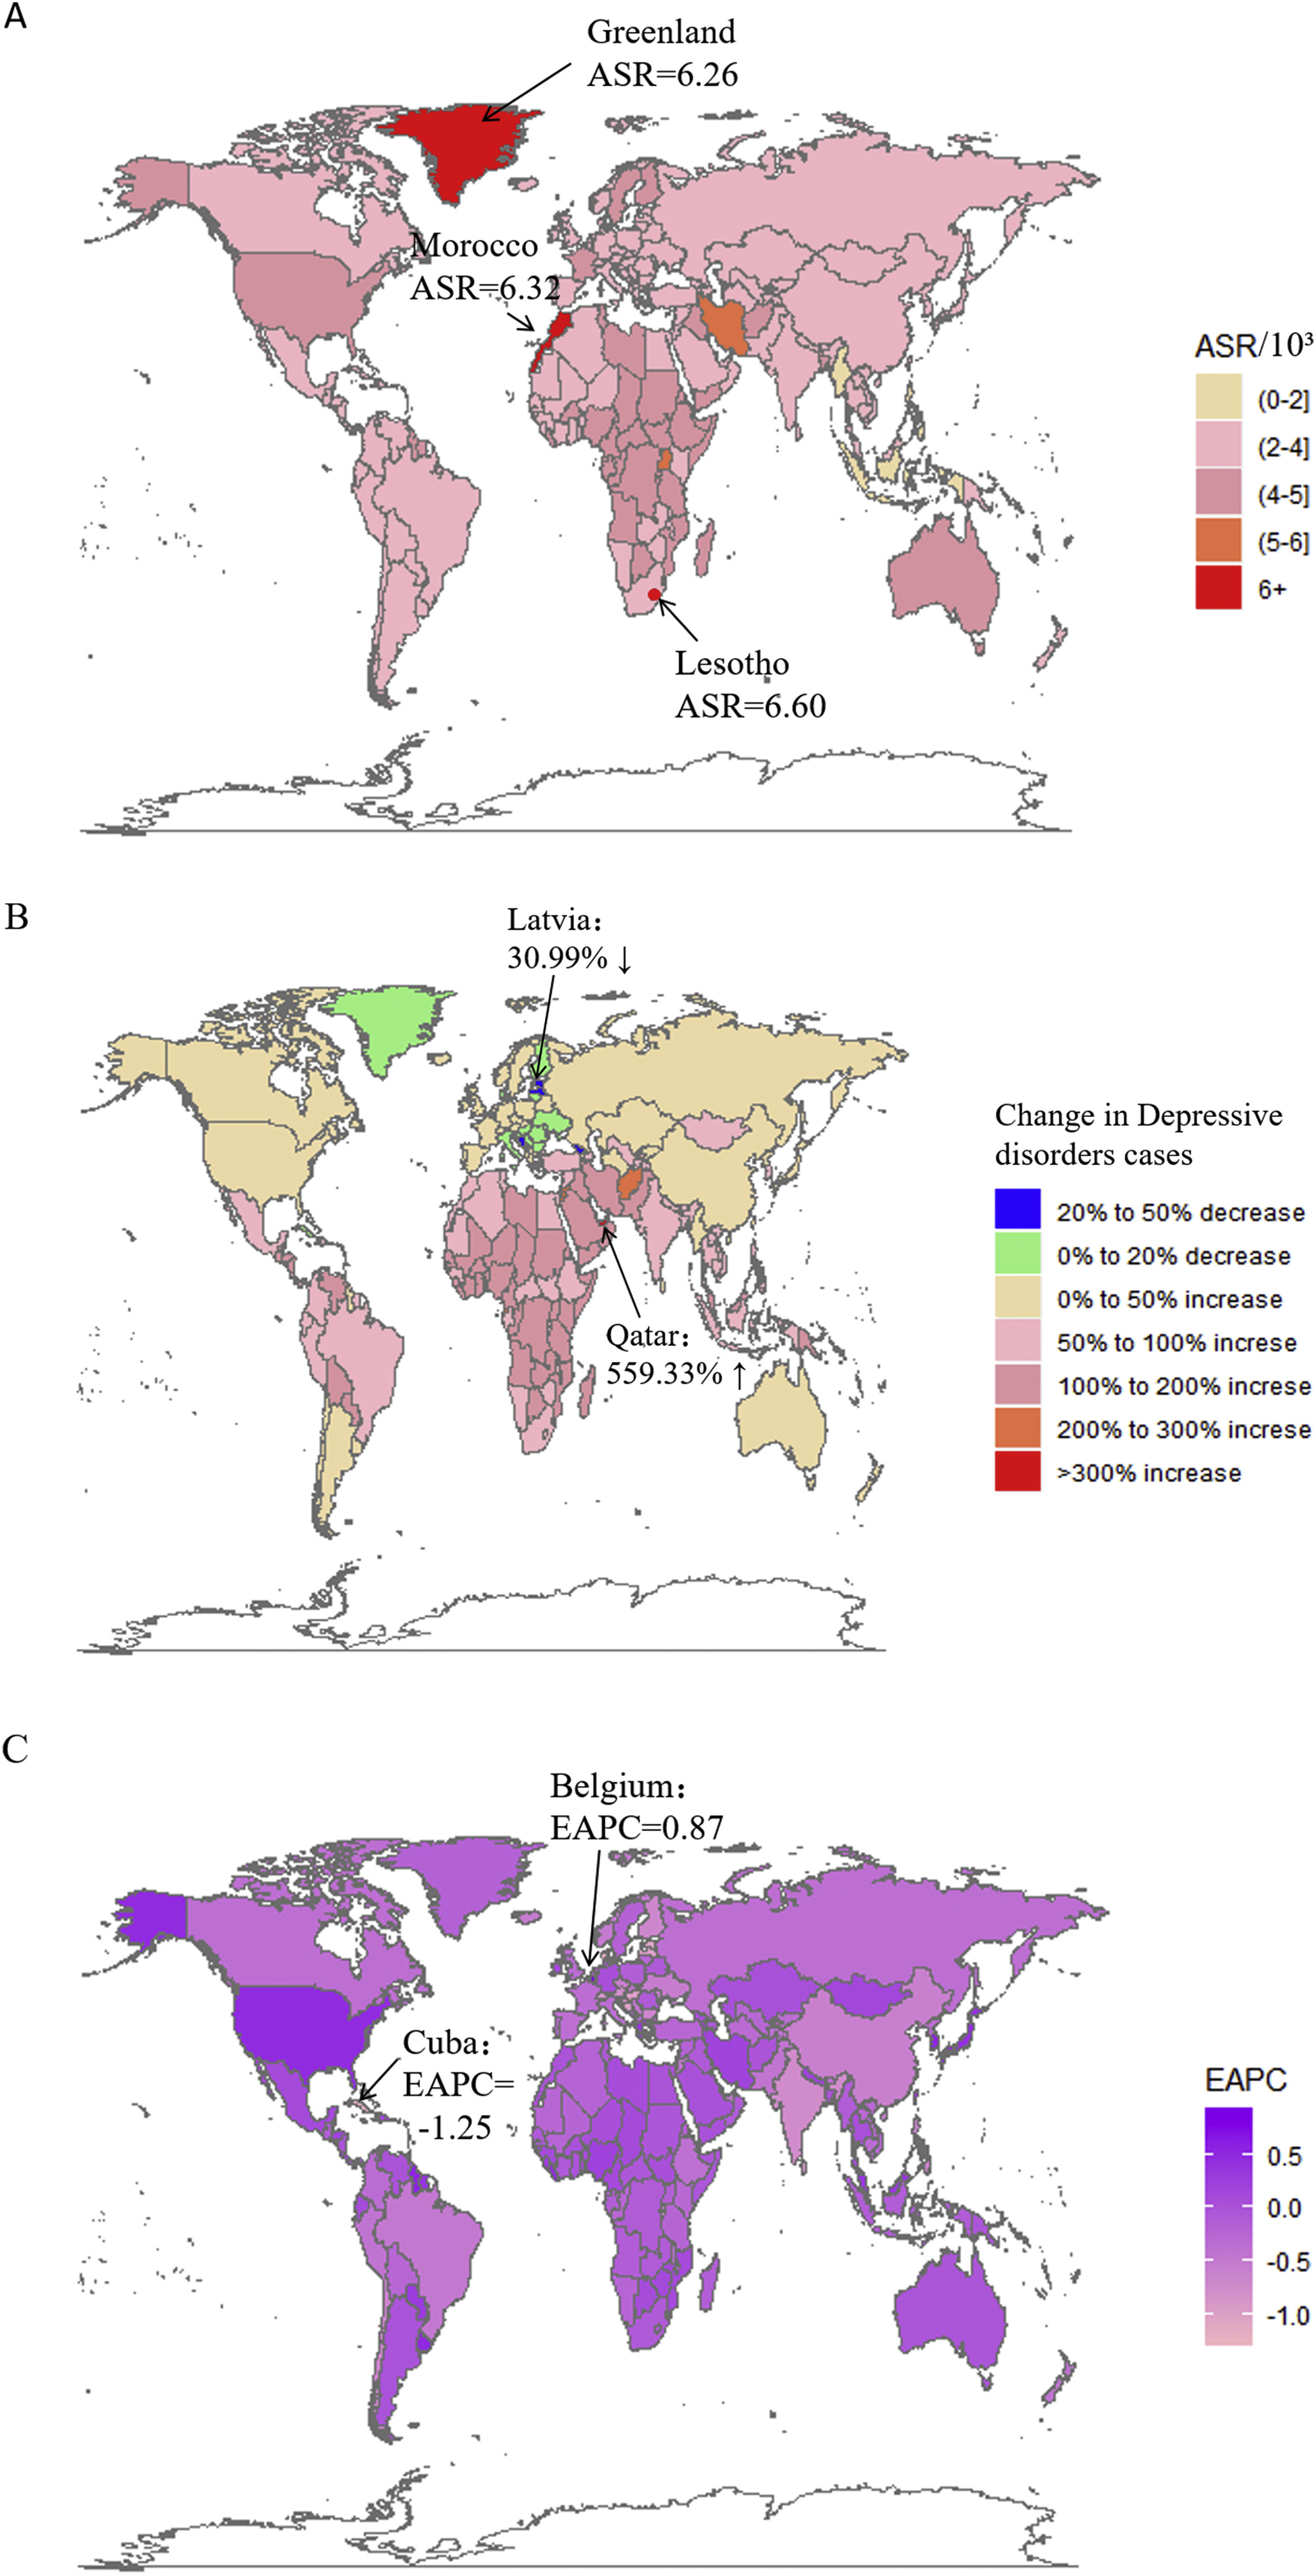
\includegraphics[scale=0.65]{./figures/depression-map-Liu-et-al-2020.jpg}
	\caption{Global depression statistics comparison between 1990 and 2017 \cite{liu2020changes}}
	\label{FigGloablDepression}
\end{figure}

\section{Objective: Tool for Depression Detection and Cross-Linguistic Evaluation}
\label{sec:ch1sec2}

The objective of our scientific study is to leverage machine learning techniques to develop a robust tool for identifying depression through textual analysis. By harnessing the power of natural language processing (NLP) and artificial intelligence (AI), we aim to create a fast and reliable tool capable of detecting signs of depression in text-based communications.

The primary goal of this endeavor is twofold. Firstly, we seek to provide a timely and accessible means of identifying individuals who may be experiencing symptoms of depression. By analyzing the language used in written communications, such as social media posts, emails, or chat messages, our tool aims to offer an initial assessment of an individual's mental well-being. This proactive approach can facilitate early intervention and support, potentially mitigating the onset of more severe depressive symptoms and their associated consequences.

Secondly, we aim to evaluate the accuracy and efficacy of our machine learning model in a cross-linguistic context. To achieve this, we will translate our dataset from English to Romanian and assess the performance of the model on both language versions. This comparative analysis will enable us to ascertain the generalizability and robustness of our tool across different languages and cultural contexts.

By undertaking this study, we hope to contribute to the advancement of computational techniques for mental health assessment and intervention. Our ultimate aim is to provide clinicians, researchers, and individuals themselves with a valuable resource for early detection and prevention of depression, ultimately fostering improved mental well-being and quality of life.